\section{The model}\label{sec4}
\subsection{Model characteristics}
The model features two types agents: sex consumers and sex producers. They are finitely lived, have rational expectations and intend to maximize future discounted utility, $E_{0}\sum_{t}^{\infty}\beta^{t}u$, subject to their respective budget constraints. I assume the function $u:[0,\infty)\to \mathbb{R}$ is strictly increasing, strictly concave and twice continuously differentiable and has a CRRA form\footnote{$u(c)=\nicefrac{c^{1-\sigma}}{(1-\sigma)}$ for sex producers and $u(c,x)=\nicefrac{c^{1-\sigma}}{(1-\sigma)}+\nicefrac{x^{1-\sigma}}{(1-\sigma)}$ for sex buyers.  Note that all agents regardless of their type share the same relative risk aversion. }, with relative risk aversion parameter $\sigma>0$.

 Agents interact in three competitive markets in this economy: The goods market, the sex market and the assets market.  
\begin{itemize}
\item There are two types of agents sex buyers ($g$) and sex producers ($-g$).  
\item From the goods market agents can obtain consumption good $c$ at price $p_{1}$\footnote{The price of the consumption will as numeraire, then $p_{1}=1$}. 
\item Non-marital risky sex $x$ is traded in the sex market for price $p_{2}=p$. Where variable $x$ is continuous.
\item Individuals can either save or borrow in the asset market by trading a non-contingent asset $a$ with endogenous return $r$.
\item Agents education can either be high or low $e=\{1,0\}$.
\item HIV status can be positive or negative $h=\{1,0\}$.
\item Labor is supplied in elastically.
\item Agents receive labor income $y(e)$, where income differs according to their education level $e$. In particular $y(1)>y(0)$.
\item The model features an exogenous component of labor income $z$ that can take two values $z^{g}$ and $z^{b}$. $z$ captures stochastic income shocks in the economy and it follows a finite state Markov chain with a given transition matrix \textit{T}: 
\end{itemize}
\begin{align*}
    \pi(s'|s) = Prob(s_{t+1}=s'|s_{t}=s)=    \begin{bmatrix}%
    p_{gg} & p_{gb}\\
    p_{bg} & p_{bb}
    \end{bmatrix}
\end{align*}
\begin{itemize}
\item Let $\gamma_{e}$ denote the survival probability of an agent with level of education $e$.
\item Let $\psi^{h}_{e}$ be the fertility rate of an individual with HIV status $h$ and education $e$.
\item Let $\lambda(x,h)$ denote the probability of getting infected with HIV. Note that the probability of infection is actually a function of the amount of risky sex ($x$) consumed by the agent. This value is determined endogenously.
\end{itemize}
Following the discussion in Section\ref{sec1}, the model intends to characterize the different stages of the HIV epidemic according to the level of education of the population. In particular, the increase in the probability of infection for the most educated in the early and final stages.\\
In line with \cite{raul}, four stages of the epidemic have been identified. 
\begin{enumerate}
\item Pre-Epidemic stage
\item Miopic stage of the epidemic
\item Difussion and maturity of the epidemic
\item Introduction of anti-retro viral drugs
\end{enumerate}
\begin{comment}
The features of each stage will be described in detail in the upcoming sections.\\

The model features additional dynamics, in the sense that it intends to capture the evolution of the HIV epidemic starting from stage one until stage four. For presentation purposes each stage characterizes a stationary equilibrium, but later on they will be linked with the intention to describe the complete evolution of the HIV epidemic.
\end{comment}


In the following sections I describe in detail the characteristics of each of the stages of the model.  

\subsection{Pre-epidemic stage}\label{pre}
There is no probability of infection, namely $\lambda(x,h)=0$ and $\psi_{e}^{h=1}=\psi_{e}^{h=0}=\psi_{e}$. Agents differ on their type $g$, assets $a$ and education level $e$.\\

\noindent\textbf{Sex Buyers:}\\
For agents of type $g$ the dynamic problem is:
\begin{align}
V(a,e,g,s;\Phi) &= \mathop{\max_{c\geq 0,x \geq 0,a' \geq 0}}  u(c,x) + \beta \gamma_{e} \sum_{s'|s}\pi(s'|s)V(a',e,g,s';\Phi') \label{eq1}\\
\mbox{s.t}\nonumber\\
c+ px +a'&= zy(e) + (1+r(\Phi))a \label{eq2}\\
a' &\leq b
\end{align}

 Agents buys non-marital risky sex $x$ at price $p$ and save or borrow $a'$ with return $r$. Agents cannot borrow amounts that exceed $b$. Note that labor is supplied in elastically and depends on their level of education $e$, then their labor income is $y(e)$, where $y(1)>y(0)$.\\
 This problem is characterized by three individual state variables ($a,e,g,s$) and one aggregate state variable $\Phi$, which represents the population distribution over the states $a,e,g,s$. The choice variables are $c,x$ and $a'$.\\
\begin{comment}
 The above problem can be written in sequential form: 
\begin{align*}
\mathop{\max_{c_{t},x_{t},a_{t+1}}}&E_{0}\sum^{\infty}_{t=0}\beta^{t}u(c_{t},x_{t})  \\
\mbox{s.t}\\ 
c_{t}+p_{t}x_{t}+a_{t+1}&=y(e)+(1+r_{t})a_{t}
\end{align*}
 \textbf{FOC's:}\\
 \begin{align*}
 \frac{\partial u(c_{t},x_{t})}{\partial x_{t}}&=-u'_{c}(c_{t},x_{t})p_{t}+u'_{x}(c_{t},x_{t})=0\\
 \frac{\partial u(c_{t},x_{t})}{\partial a_{t+1}}&=-u'_{c}(c_{t},x_{t})+u'_{c}(c_{t+1},x_{t+1})(1+r_{t})\beta=0
 \end{align*}
 Given the price system $\{p_{t}\}_{t=0}^{\infty},\{r_{t}\}_{t=0}^{\infty}$ the solution is characterized by the sequence of allocations $\{c_{t}\}_{t=0}^{\infty}, \{x_{t}\}_{t=0}^{\infty}, \{a_{t}\}_{t=0}^{\infty}$ such that they solve the above maximization problem.\\
\end{comment}

\noindent \textbf{Sex Producers:}\\
For agents of type $-g$ the dynamic problem is:
\begin{align}
V(a,e,-g,s;\Phi) &= \mathop{\max_{c\geq 0, 1\geq l\geq 0,a' \geq 0}}  u(c) + \beta \gamma_{e} \sum_{s'|s}\pi(s'|s)V(a',e,-g,s';\Phi') \label{eq3}\\
\mbox{s.t}\nonumber\\
c +a'&= pl^{\alpha}+zy(e)(1-l) + (1+r(\Phi))a \label{eq4}\\
a' &\leq b
\end{align}
Note that for these agents, extra marital risky sex ($x$) does not generate any utility, then the utility function only depends on the amount of consumed ($c$). Additionally, these agents produce sex with a decreasing return to scale production function $x=l^{\alpha}$ where $\alpha\in(0,1)$. In other words, these agents produce non-marital risky-sex $x$ using time $l$ and sell it a price $p$. Where $l$ is the fraction of labor dedicated to the production of extramarital risky sex, the remaining labor ($1-l$), which is not allocated to sex production, is sold in the market for labor income $y(e)$. As before, agents are allowed to save or borrow assets $a$ at rate $r$.\\

\begin{comment}
\noindent The above problem can be written in sequential form: 
\begin{align*}
\mathop{\max_{c_{t},l_{t},a_{t+1}}}&E_{0}\sum^{\infty}_{t=0}\beta^{t}u(c_{t})  \\
\mbox{s.t}\\ 
c_{t}+a_{t+1}&=p_{t}l_{t}^{\alpha}+y(e)(1-l_{t})+(1+r_{t})a_{t}
\end{align*}
 \textbf{FOC's:}\\
 \begin{align*}
 \frac{\partial u(c_{t})}{\partial l_{t}}&=-u'_{c}(c_{t})(\alpha p_{t} u^{\alpha-1}-y(e))=0\\
 \frac{\partial u(c_{t})}{\partial a_{t+1}}&=-u'_{c}(c_{t})+u'_{c}(c_{t+1})(1+r_{t})\beta=0
 \end{align*}
 Given the sequence of prices $\{p_{t}\}_{t=0}^{\infty},\{r_{t}\}_{t=0}^{\infty}$ the solution are the sequences of allocations $\{c_{t}\}_{t=0}^{\infty},\{l_{t}\}_{t=0}^{\infty}, \{l_{t}\}_{t=0}^{\infty}, \{a_{t}\}_{t=0}^{\infty}$ that solve  the agent's problem.\\
 
\end{comment}


 \subsection*{The aggregate state variable and transition function}
\noindent The aggregate state variable evolves according to:
\begin{align}
\Phi'=F(\Phi)
\end{align} 
Where the function $F:\mathcal{M}\to\mathcal{M}$ is the aggregate law of motion, mapping distributions to distributions. $F$ summarizes how agents move within the distribution of assets , education and type from one period to the next, however this is exactly what a transition function tell us. \\
\noindent Define the transition function $\mathcal{Q}:\mathcal{Z}\times\mathcal{B(Z)}\to[0,1]$ by: 
\begin{align*}
Q((a,e,g,s)(\mathcal{A},\mathcal{E},\mathcal{G},\mathcal{S})) &= \left\{
\begin{tabular}{clc}
$\gamma_{e}$ & if      & $a(a,e,g,s;\Phi) \in \mathcal{A} $\\
0 & else & 
\end{tabular}
\right.\\
\forall \,\,\,(a,e,g,s)&\in\mathcal{Z}\,\,\,\mbox{and}\,\,\,(\mathcal{A,E,G,S})\in{\mathcal{B(Z)}}
\end{align*}
Where $\mathcal{Z}$ consists of all n-tuples of $A\times E\times G\times S$. \\
Define $\mathcal{B(Z)}$ as the set of Borel sets on $\mathcal{Z}$, in particular $\mathcal{A,E,G,S}\in\mathcal{B(Z)}$ where $\mathcal{A,E,G,S}$ are projections of $\mathcal{Z}$ over the spaces $A,E,G$ and $S$ respectively. Let $\mathcal{P}$ be a probability measure on $\mathcal{B(Z)}$, then $\mathcal{P}: \mathcal{B(Z)}\to[0,1]$.\\
Then the evolution of the asset distribution is:
\begin{align}
\Phi'(\mathcal{A,E,G,S}) = F(\Phi) (\mathcal{A,E,G,S})= \int_{a,e,g,s} Q((a,e,g,s)(\mathcal{A,E,G,S})) d \Phi\\+\psi_{e}\Phi((a',e,g,s')(\mathcal{A,E,G,S}))
\end{align}
Which is the fraction of people with assets in $\mathcal{A}$, education $\mathcal{E}$, type $\mathcal{G}$ and states in $\mathcal{S}$ as measured by $\Phi$, that transit to ($\mathcal{A,E,G,S}$) as measured by $\mathcal{Q}$. The last term accounts for the new born. Population of each group increases according to their respective fertility rate $\psi_{e}$. It important to note that individuals of a certain type give birth to people of the same type.
 \subsection*{Solution to the recursive problem}
 Given prices $p,r$ the solution to the recursive problem of agents $g$ and $-g$  are the policy functions $a'(a,e,g,s;\Phi), x(a,e,g,s;\Phi), c(a,e,g,s;\Phi), l(a,e,g;\Phi)$ that induce a stationary distribution $\Phi(\mathcal{A,E,G,S})$ over the set of state variables. Where $\Phi$ is the aggregate state variable.
 \subsection*{Stationary equilibrium}
 The \textit{stationary equilibrium of the Pre-Epicemic stage} is:
 \begin{itemize}
 \item An interest rate $r$ and price $p$
 \item Policy functions $a'(a,e,g,s;\Phi), x(a,e,g,s;\Phi), c(a,e,g,s;\Phi), l(a,e,g,s;\Phi)$
 \item A stationary distribution $\Phi(\mathcal{A,E,G,S}) $
 \end{itemize}
 Such that:
 \begin{enumerate}[label=\alph*]
 \item Given $r$ and $p$ the policy functions  $a'(a,e,g,s;\Phi), x(a,e,g,s;\Phi), c(a,e,g,s;\Phi), l(a,e,g,s;\Phi)$ solve the sex buyers and sex producers problem respectively. 
 \item The stationary probability distribution $\Phi'(\mathcal{A,E,G,S})$ is induced by the optimal policy $a'(a,e,g,s;\Phi)$.
 \item All markets clear. 
  \end{enumerate}
 \begin{align*}
\int_{a,e,g,s} a'(a,e,g,s;\Phi) d\Phi &= 0 \\
\int_{a,e,g,s} x(a,e,g,s;\Phi) d \Phi &= \int_{a,e,-g,s} x(a,e,-g,s;\Phi) d\Phi
\end{align*} 
That is, there is zero net supply of assets, the sex markets clear and the consumption market clears by Walras law. 
\subsection*{Computing the stationary equilibrium for the Pre-epidemic stage}
\noindent \textbf{Calibration of the parameters:}\\
\begin{center}
\begin{longtable}{ccc}
\caption{List of parameters}\\%
\hline%
\multicolumn{1}{c}{\textbf{\LaTeX}} &
\multicolumn{1}{c}{\textbf{Description}} &
\multicolumn{1}{c}{\textbf{Value}}\\%
\hline\hline%
\endfirsthead
\multicolumn{3}{c}{{\tablename} \thetable{} -- Continued}\\%
\hline%
\multicolumn{1}{c}{\textbf{\LaTeX}} &
\multicolumn{1}{c}{\textbf{Description}}\\%
\hline\hline%
\endhead
${\beta}$ & Discount factor & 0.99\\
${\alpha}$ & Labor share of income & 0.1\\
${\sigma}$ & Risk aversion & 1.5 \\
${\gamma_{e=1}}$ & Survival rate educated (\%) & 99\\
${\gamma_{e=0}}$ & Survival rate less educated (\%) & 98\\
${\psi_{e=1}}$ & Fertility rate educated (\%) & 3\\
${\psi_{e=0}}$ & Fertility rate less educated (\%) & 6\\
${\omega}$ & People with at least secondary education (\%) & 32\\
${y_{e=1,t}}$ & Endowment educated at period $t$ & 0.75\\
${y_{e=0,t}}$ & Endowment less educated at period $t$ & 0.56\\
$s^{g}$ & Positive income shock & 1.06\\
$s^{b}$ & Negative income shock & 0.94\\
$p_{gg}$ & Transit probability from $z_{g}$ to $z_{g}$ & 0.95\\
$p_{gb}$ & Transit probability from $z_{g}$ to $z_{b}$ & 0.05\\
$p_{bg}$ & Transit probability from $z_{b}$ to $z_{g}$ & 0.05\\
$p_{bb}$ & Transit probability from $z_{b}$ to $z_{b}$ & 0.95\\
$a_{min}$ & Lower limit of the asset grid & -5 \\
$a_{max}$ & Upper limit of the asset grid & 8\\
$n$ & number of nodes in the asset grid& 7\\

\hline%
\end{longtable}
\end{center}

The values for $\beta, \alpha, \sigma$ are standard in the literature. The survival rate $\gamma_{e}$ and fertility rate were $\psi$ are data form the World Bank, Sustainable Development Indicators for Malawi. Additionally the share of people with at least secondary education has been taken from DHS\footnote{Demographic and health survey} data for Malawi.\\

$b$ is set to be the models natural borrowing constrain, this means that agents do not have any kind of liquidity constraint as in the pre-epidemic stage the natural borrowing constraint is never binding. Additionally $a_{min}$ has been chosen low enough to surpass the natural borrowing constraint $b$ set by the model. Consequently $a_{max}$ has been chosen large enough so that agents do not hold assets in excess of $a_{max}$ in the stationary equilibrium. The choice of $n$ is arbitrary, higher numbers of $n$ incur in longer computing time.

\noindent \textbf{\textit{Algorithm No.1}: Computation of the stationary equilibrium:}\\

\noindent\textit{Step 1: Make initial guesses of price $p$ and interest rate $r$.\\
Step 2: Compute the agents decision rules.\\
Step 3: Compute the stationary distribution of assets (follow Algorithm No.2).\\
Step 4: Compute aggregate assets demand and aggregate sex demand. Check the aggregate consistency conditions.\\
Step 5: If conditions are not met, update $p$ and $r$ and return to Step 2. 
}\\

Keep in mind that \textit{Algorithm No.1} is generic enough so that it can also be applied to compute the stationary equilibrium of any stage of the HIV epidemic.\\

For the computation of the decision rules I make use of value function iteration with linear interpolation as described in any computational methods text book\footnote{Refer to \cite{mauss}, \cite{judd}, \cite{sargent}}. For the value function iteration procedure it is necessary to choose a grid over the asset space $A=\{a_{1}=a_{min},...,a_{n}=a_{max}\}$ where $a_{min}$ and $a_{max}$ are the values chosen in the calibration. \\

\noindent\textbf{\textit{Algorithm No.2}: Computation of the invariant distribution:}\\

\noindent\textit{Step 1: Choose a grid over the asset space $A=\{a_{1}=a_{min},...,a_{n}=a_{max}\}$.\\
Step 2: Set a time iteration counter $t=0$ and choose an initial (discrete) density function $\phi_{0}(a,e,g,s)$ over the state space.\\
Step 3: Initialize $\phi_{t+1}(a',e,g,s')$\footnote{$\phi_{t+1}$ is of dimensions $n\times (m*w*q)$, where $m=2$, $w=2$ and $q=2$ since education, type and stochastic states can only be of two sorts.} and compute the optimal next period wealth $a'$ with the help of the decision rule.\\
Step 4: For all $a'\in A$, $e \in E$, $g \in G$ and $s \in S$compute the following expression:}
\begin{align}
    \phi_{t+1}(a',e,g,s')=\sum_{a,e,s}\sum_{s'|s}\textbf{1}_{a'\in\mathcal{A}}\gamma_{e}\pi(s'|s)\phi_{t}(a,e,g,s) + \psi_{e}\phi_{t}(a',e,g,s')
\end{align}
\textit{
Step 5: If $|\phi_{t+1}-\phi_{t}|<exp(-12)$ stop, otherwise set $\phi_{t}=\phi_{t+1}$ and return to Step 3.}\\

For simplicity reasons the grid chosen for \textit{Algorithm No.2} is the same as the grid chosen for the value function iteration procedure in \textit{Algorithm No.1}, otherwise if the grid would be finer it would be necessary to include the probabilities of $a'(a,e,g,s)$ falling between the respective points in the grid.\\

For \textit{Step2} of \textit{Algorithm No.2} I choose the uniform distribution as the initial values of the distribution. The algorithm should converge regardless of the choice of the initial distribution. 


%\subsection*{Computing the dynamics for the pre-epidemic stage}


\subsection*{Results}
\begin{table}[H]
\caption{Equilibrium prices}%
\begin{center}
\begin{tabular}{r|c}
\hline%
\textbf{Price of sex} &0.32\\
\hline
\textbf{Interest Rate} & 9.25\%\\
\hline%
\end{tabular}
\end{center}
\end{table}

%\begin{figure}[t!]

\begin{figure}[H]
\caption{Equilibrium}
\hspace{-2.0cm}
\begin{center}
\begin{tabular}{cc}
\multicolumn{1}{c}{(a) Sex Market} &  
\multicolumn{1}{c}{(b) Asset Market} \\
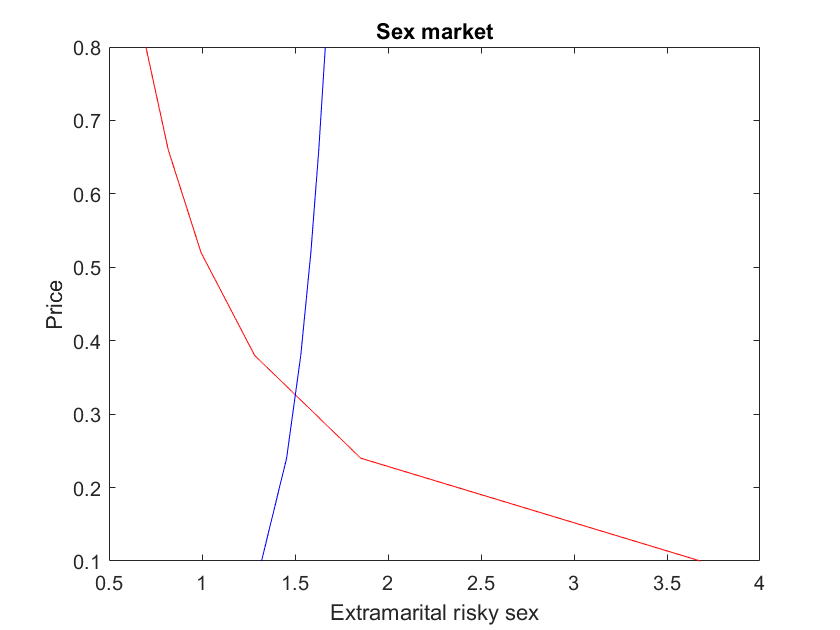
\includegraphics[angle=0,width=.5\textwidth]{figures/FIG14.png}   & 
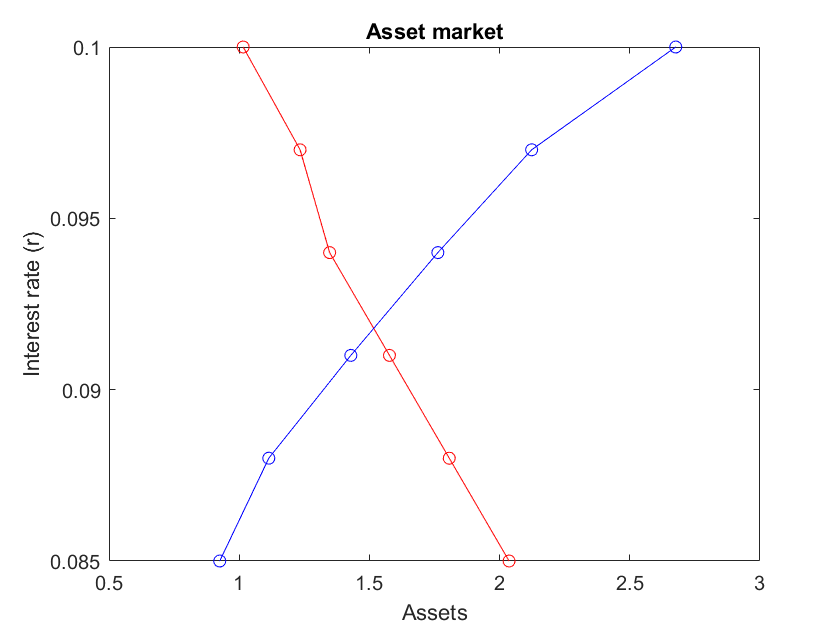
\includegraphics[angle=0,width=.5\textwidth]{figures/FIG15.png} 

%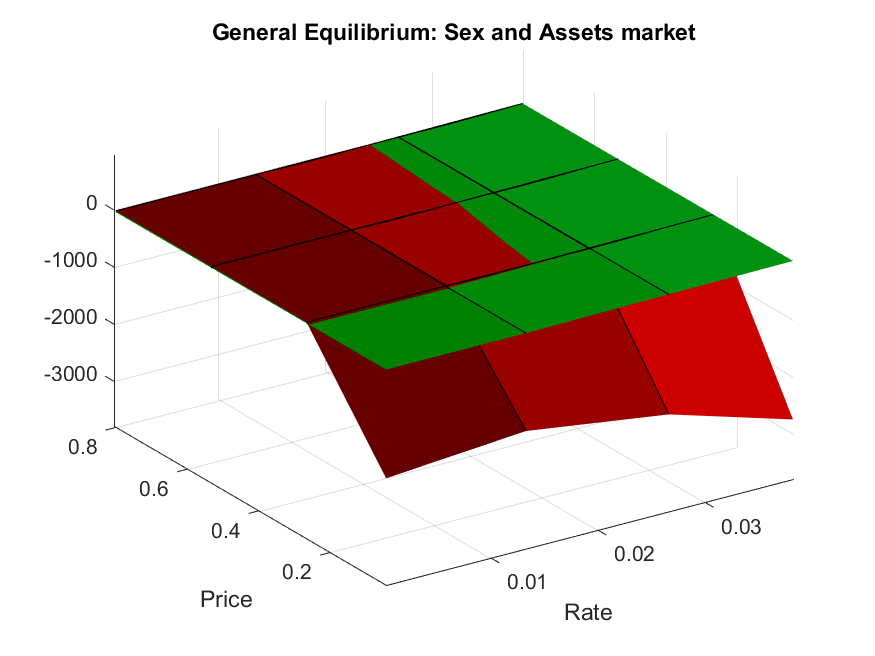
\includegraphics[angle=0,width=.5\textwidth]{figures/FIG_EQUILIBIUM3.png} 
\end{tabular}
\end{center}
\label{fig:6}
\end{figure}

\begin{figure}[H]
\caption{Distributions}
\hspace{-2.0cm}
\begin{center}
\begin{tabular}{cc}
\multicolumn{1}{c}{(a) Asset Distribution} &  
\multicolumn{1}{c}{(b) Income Distribution} \\
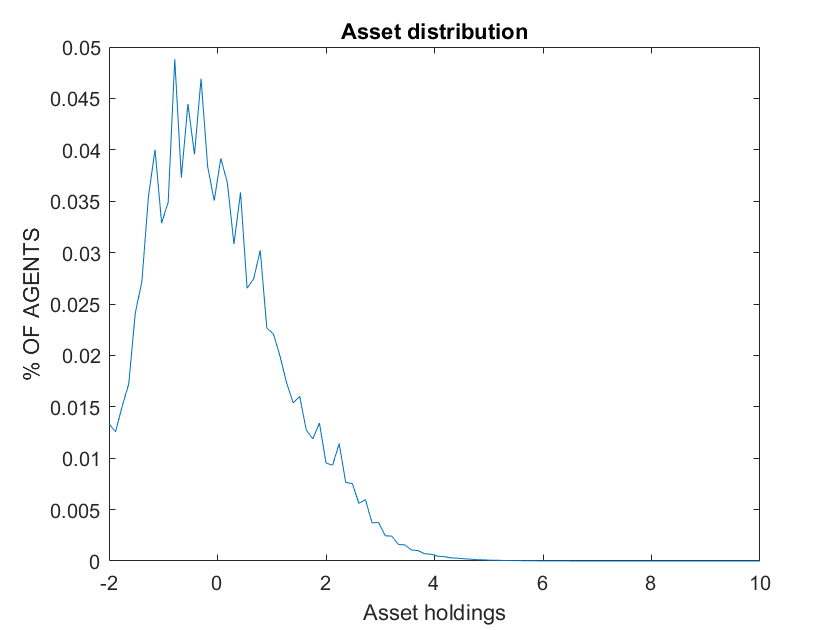
\includegraphics[angle=0,width=.5\textwidth]{figures/FIG9.png}   & 
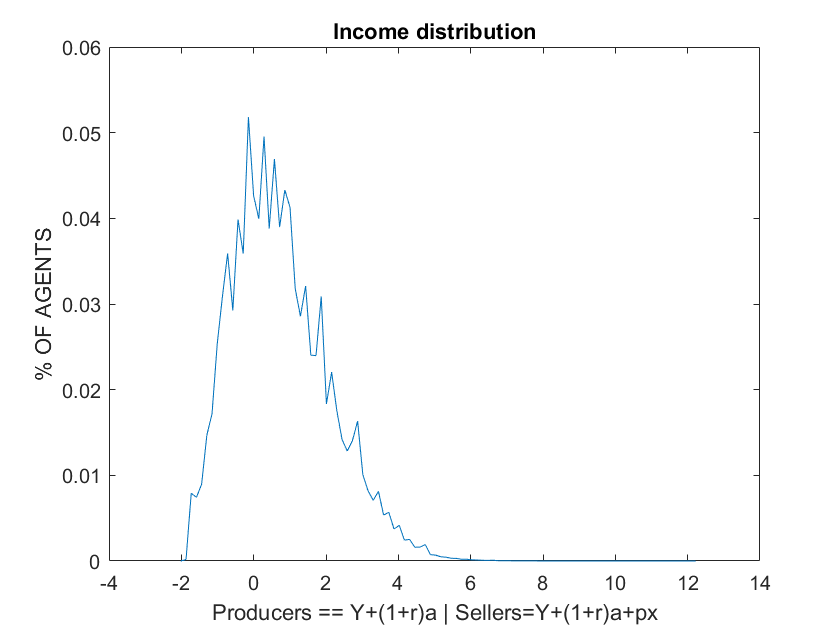
\includegraphics[angle=0,width=.5\textwidth]{figures/FIG10.png} 
\end{tabular}
\end{center}
\label{fig:4}
\end{figure}

\begin{figure}[H]
\caption{Policy Functions Educated Buyers}
\hspace{-2.0cm}
\begin{center}
\begin{tabular}{cc}
\multicolumn{1}{c}{(a) Value function} &  
\multicolumn{1}{c}{(b) Assets function} \\
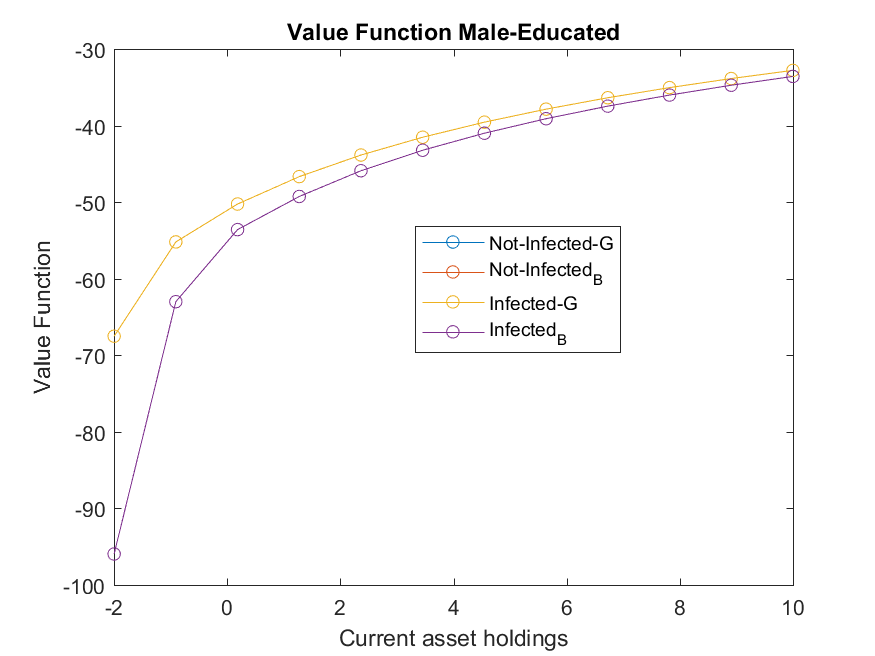
\includegraphics[angle=0,width=.5\textwidth]{figures/FIG1.png}   & 
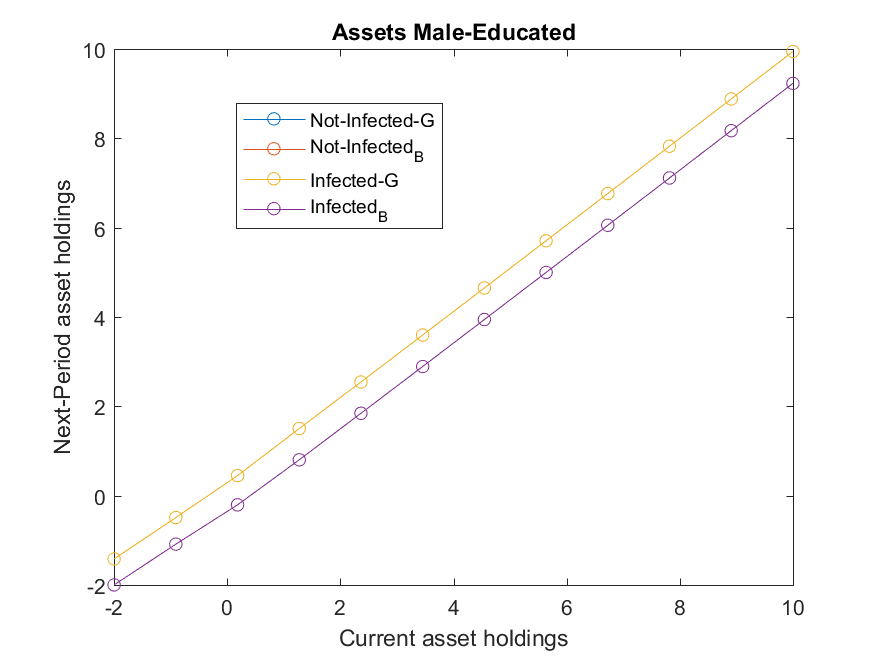
\includegraphics[angle=0,width=.5\textwidth]{figures/FIG3.png} \\
\multicolumn{1}{c}{(c) Consumption function} &  
\multicolumn{1}{c}{(d) Sex consumption function } \\
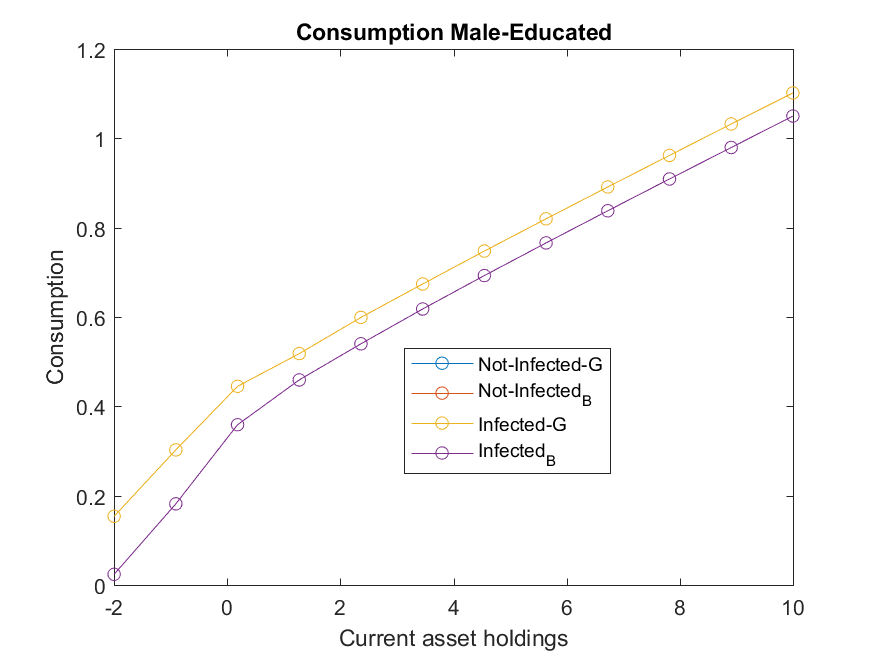
\includegraphics[angle=0,width=.5\textwidth]{figures/FIG2.png}   & 
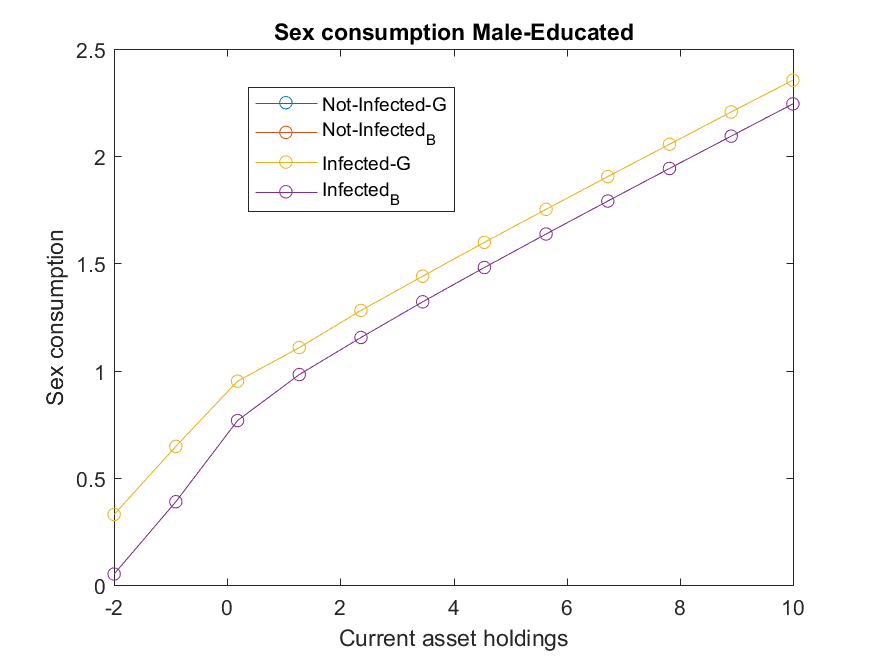
\includegraphics[angle=0,width=.5\textwidth]{figures/FIG4.png} \\
%\multicolumn{1}{c}{(a) Value function} &  
%\multicolumn{1}{c}{(b) Assets function} \\
\end{tabular}
\end{center}
\label{fig:2}
\end{figure}

\begin{figure}[H]
\caption{Policy Functions Educated Sellers}
\hspace{-2.0cm}
\begin{center}
\begin{tabular}{cc}
\multicolumn{1}{c}{(a) Value function} &  
\multicolumn{1}{c}{(b) Asset function} \\
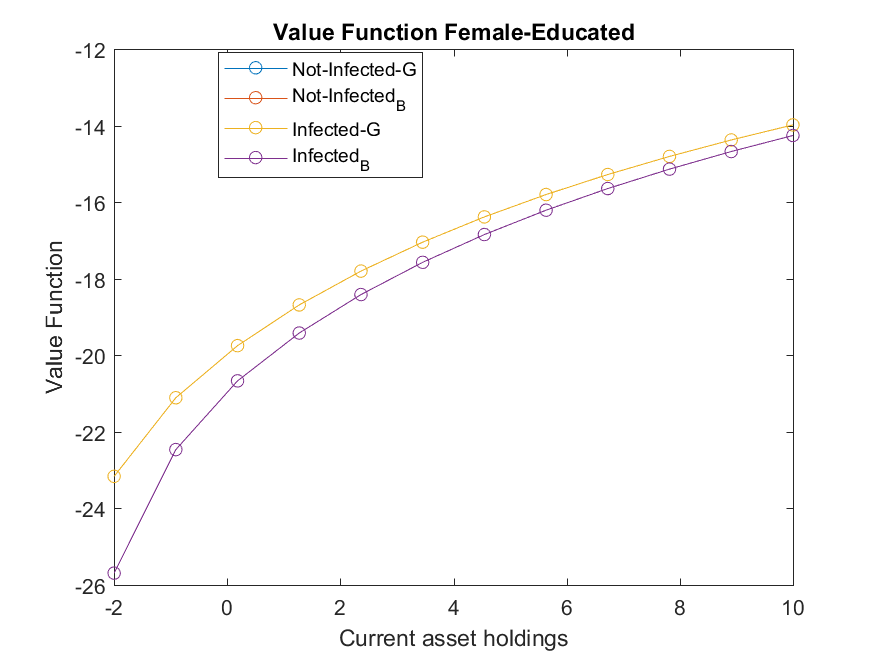
\includegraphics[angle=0,width=.5\textwidth]{figures/FIG5.png}   & 
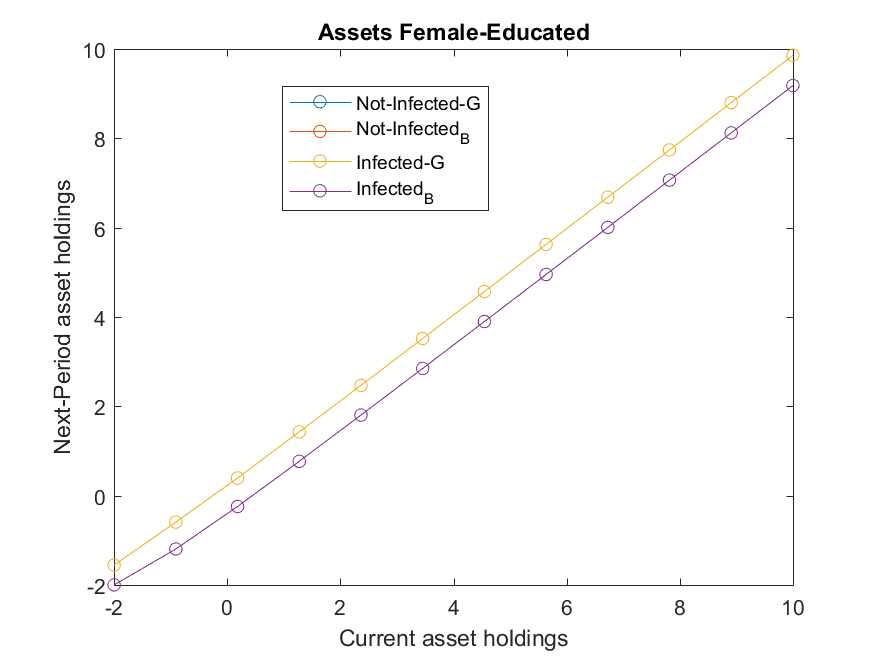
\includegraphics[angle=0,width=.5\textwidth]{figures/FIG7.png} \\
\multicolumn{1}{c}{(c) Consumption function} &  
\multicolumn{1}{c}{(d) Sex Production function } \\
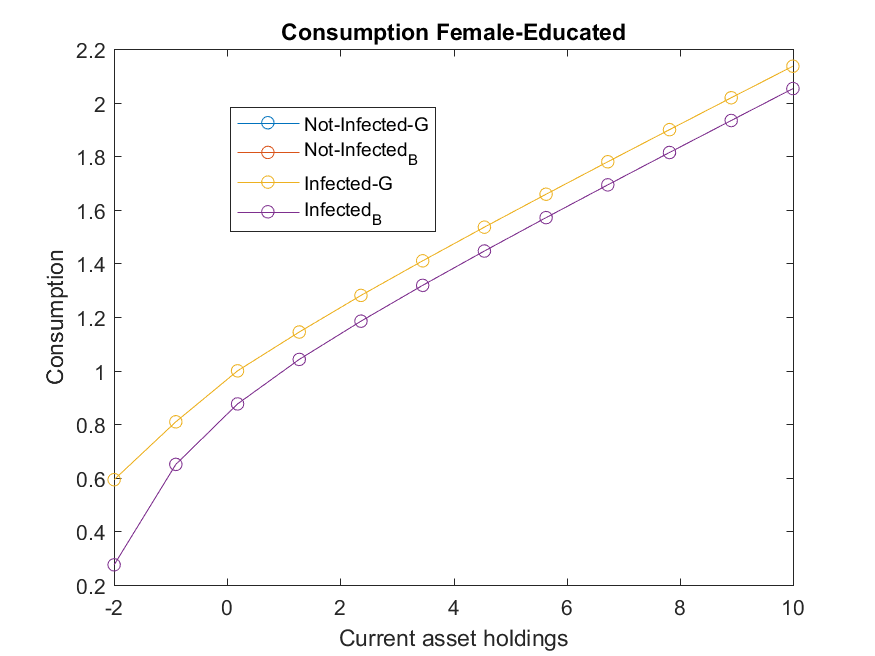
\includegraphics[angle=0,width=.5\textwidth]{figures/FIG6.png}   & 
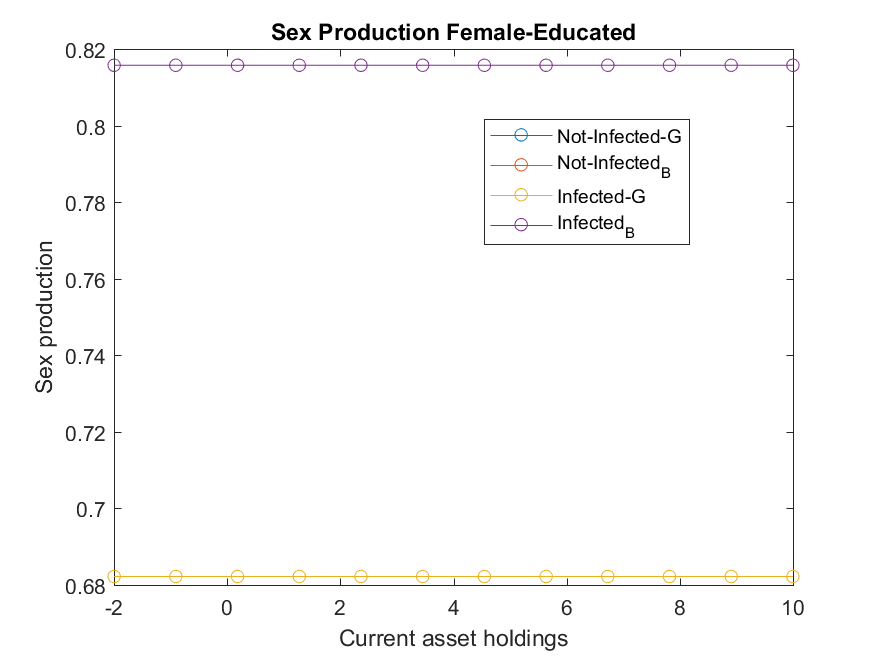
\includegraphics[angle=0,width=.5\textwidth]{figures/FIG8.png} \\
\end{tabular}
\end{center}
\label{fig:3}
\end{figure}



\begin{figure}[H]
\caption{Comparison plots}
\hspace{-2.0cm}
\begin{center}
\begin{tabular}{cc}
\multicolumn{1}{c}{(a) Asset Policy Functions} &  
\multicolumn{1}{c}{(b) Consumption Policy Functions} \\
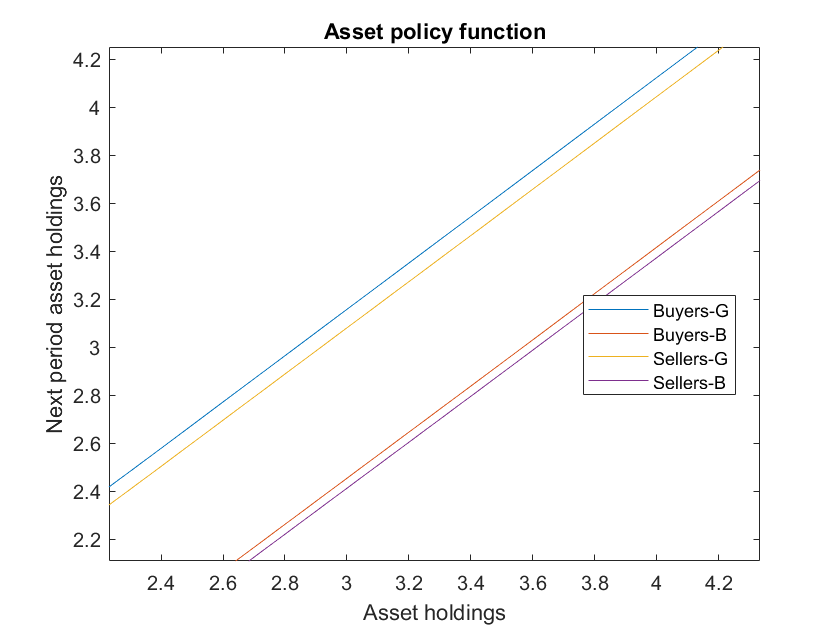
\includegraphics[angle=0,width=.5\textwidth]{figures/FIG11.png}   & 
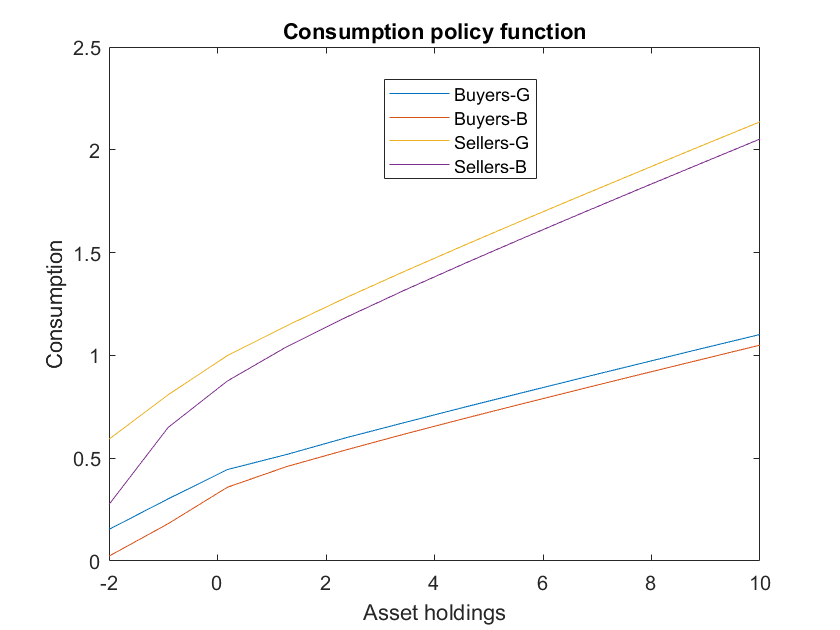
\includegraphics[angle=0,width=.5\textwidth]{figures/FIG12.png}\\ 
\multicolumn{2}{c}{(c) No Capital Income} \\  
%\multicolumn{2}{c}{(d) Equilibrium(repeated)} \\
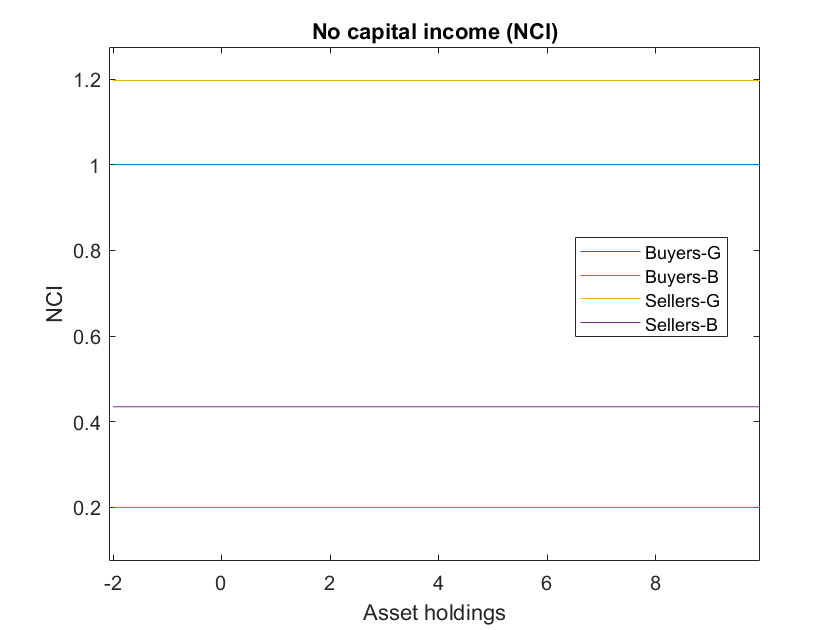
\includegraphics[angle=0,width=.5\textwidth]{figures/FIG13.png} 
%& 
%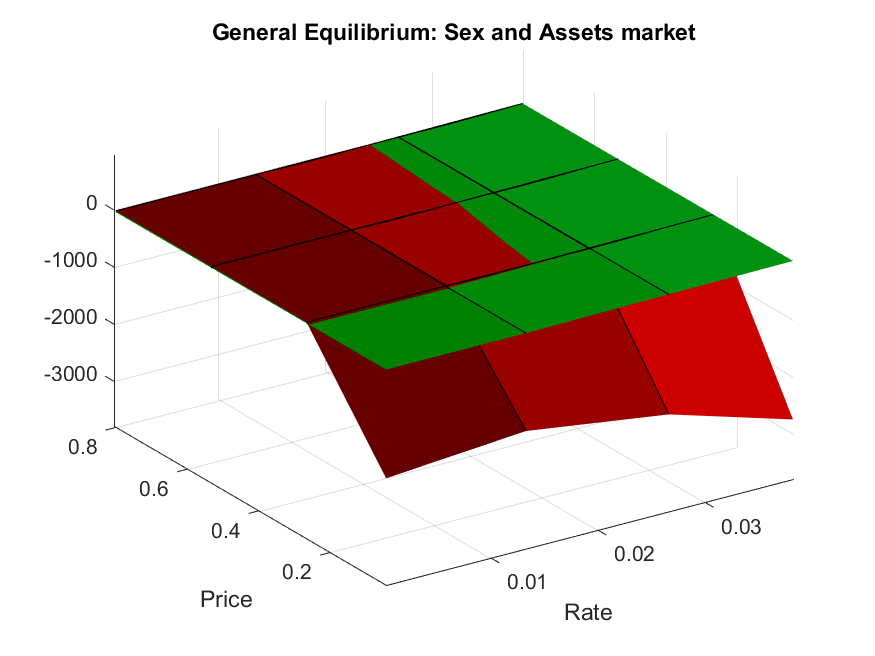
\includegraphics[angle=0,width=.5\textwidth]{figures/FIG_EQUILIBIUM3.png} 
\end{tabular}
\end{center}
\label{fig:5}
\end{figure}

\begin{figure}[H]
\caption{General equilibrium surface plots}
\hspace{-2.0cm}
\begin{center}
\begin{tabular}{cc}
\multicolumn{1}{c}{(a) Excess demand of Sex} &  
\multicolumn{1}{c}{(b) Excess demand of Assets} \\
%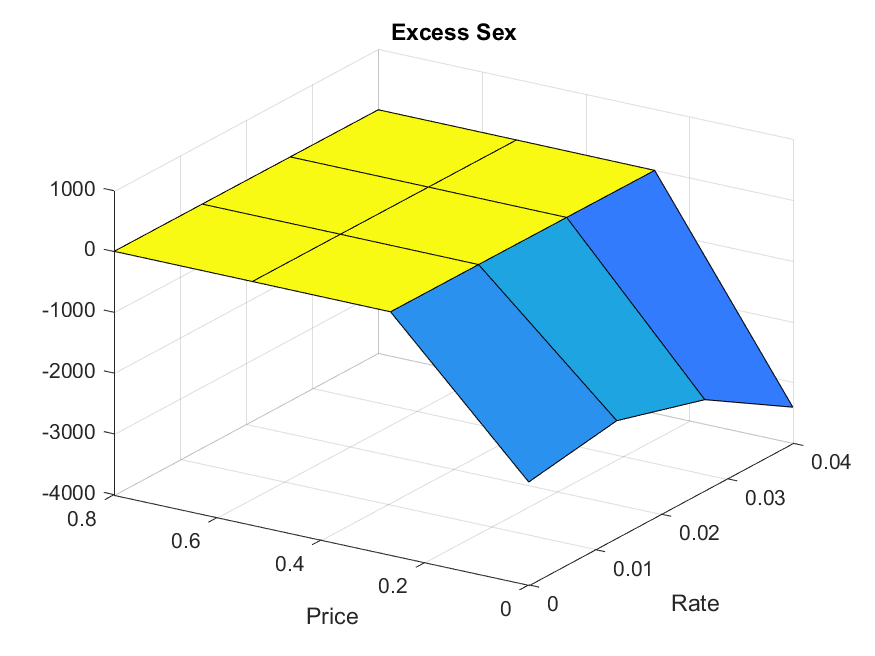
\includegraphics[angle=0,width=.5\textwidth]{figures/FIG_EQUILIBIUM2.png}   & 
%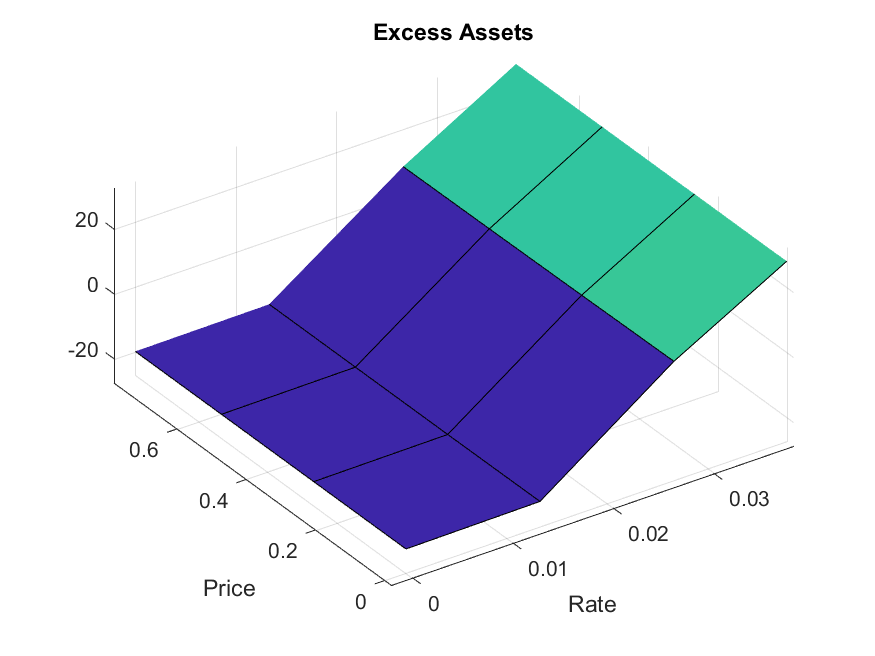
\includegraphics[angle=0,width=.5\textwidth]{figures/FIG_EQUILIBIUM1.png}\\ 
\multicolumn{2}{c}{(c) Equilibrium} \\  
%\multicolumn{2}{c}{(d) Equilibrium(repeated)} \\
%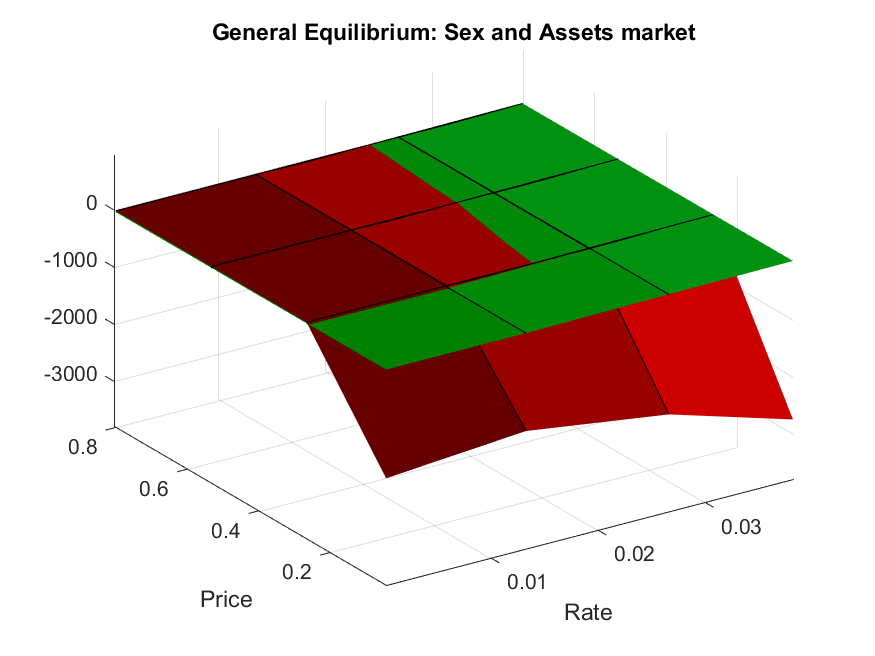
\includegraphics[angle=0,width=.5\textwidth]{figures/FIG_EQUILIBIUM3.png} 
%& 
%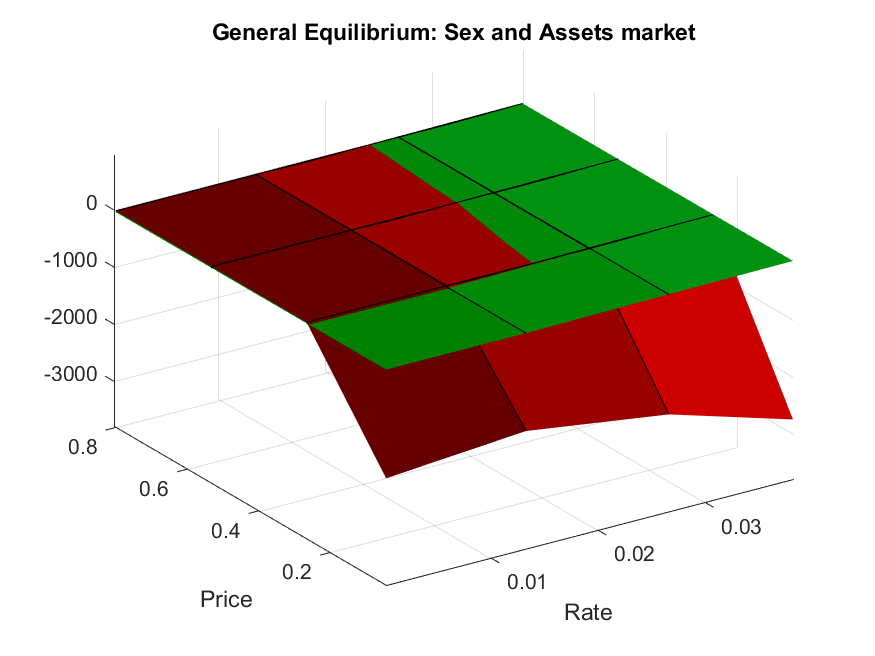
\includegraphics[angle=0,width=.5\textwidth]{figures/FIG_EQUILIBIUM3.png} 
\end{tabular}
\end{center}
\label{fig:1}
\end{figure}